\chapter{Teknologi}
\label{ch:technology}
Dette kapittelet redegjør kort for de ulike teknologiene som er relevante
for avstandsoppfølging i dette prosjektet: protokoller og metoder
for kommunikasjon, skyteknologi og skyløsninger, plattformer for elektronikkprototyping og sensorer og aktuatorer.

\section{Protokoller og kommunikasjon}
Delkapittelet tar for seg \gls{mqtt} som kjører
på \gls{tcp}, trådløsstandarden \gls{ble} og sikkerhetsutfordringer med \gls{ble} og seriell kommunikasjon og \gls{gpio} for kommunikasjongrensesnitt mellom elektronikk.

\subsection{MQTT} % WebSockets
\iffalse
WebSockets er en protokoll for applikasjonslaget på toppen av \gls{tcp}
som gjør det mulig med toveiskommunikasjon gjennom en enkelt \gls{tcp}-socket.
I følge \citet{rfc6455} ble protokollen introdusert for å unngå tungvint \gls{http}-polling.

Websockets har et lite klient-\gls{api} der en kan få en god oversikt ved å lese
kodesnutt \ref{lst:websockets}. \gls{api}-et er basert på eventer, og forskjellige \textit{callback}-funksjoner
vil bli kalt når det skjer noe spesielt, for eksempel når en ny melding er sendt til klienten eller
når tilkoblingen lukkes. Protokollen støtter \gls{tls}, og er implementert i alle de største nettleserne.
Den kan også brukes i andre miljøer og språk med gode nettverksbyggeklosser.

\begin{minipage}{\linewidth}
\begin{lstlisting}[frame=single, language=JavaScript,
    caption=WebSockets: JavaScript-eksempelkode, label=lst:websockets]
    //Initiate a new secure WebSocket connection with TLS
    const ws = new WebSocket("wss://address:port");

    //Attach functions to event handlers
    ws.onmessage = function(e) {
        var data = JSON.parse(e.data);
    };

    ws.onclose = function() {} //connection is closed

    ws.onerror = function() {} //something went wrong
    
    ws.onopen = function() {
        ws.send(JSON.stringify({ msg: "Hello, World" }));
    }
\end{lstlisting}
\end{minipage}
\fi

\gls{mqtt} er et lettvekt og meldingbasert klient-tjener-protokoll bygget for \gls{iot}-kommunikasjon
og \gls{m2m} \citep{mqtt_standard}. Den er designet for å bruke lite data og fungere bra på
dårlige nettverksforbindelser. \gls{mqtt} kjører direkte på \gls{tcp}/IP eller over WebSockets.

Protokollen er basert på \textit{publish-subscribe}-meldingsmønsteret. En klient kan publisere hva som helst til
et emne (streng, eller liste av strenger). En annen klient som abonnerer på det samme emne
vil motta datapakken fra den andre klienten. Dette gir de følgende klientmetodesignaturene for \gls{mqtt}
i kodesnutt \ref{lst:mqtt}:

\begin{lstlisting}[frame=single, caption=Klientside-API for MQTT, label=lst:mqtt]
    connect(mqtt://address:port)
    subscribe(topic: String | list of topics: String)
    unsubscribe(topic: String | list of topics: String)
    publish(topic: String, payload: String/binary)
    onMessageReceived(topic: String, payload: String/binary)
    close()
\end{lstlisting}

\gls{mqtt}-\textit{brokeren} tar i mot og behandler innkommende klienttilkoblinger og stopp av abonnement. I tillegg
mottar den meldinger og sender meldinger videre til klienter som abonnerer på et emne. MQTT kjører på port 1883, mens
MQTT over \gls{tls} kjører på port 8883.

\subsection{Bluetooth Low Energy}
\gls{ble}, tidligere markedsført som Bluetooth Smart, ble en del av Bluetooth-standarden fra versjon 4. BLE er egnet
for trådløs direktekommunikasjon mellom små enheter med lavt strømforbruk.

Bluetooth-standarden opererer med applikasjonsprofiler som beskriver hvordan man skal samhandle med
en Bluetooth-enhet. Profilene er bygget på \textit{generic attribute profile} (GATT), en spesifikasjon for å sende og motta
små databiter (attributter) over en datalink. %\todo{Kilde? \url{https://www.bluetooth.com/specifications/generic-attributes-overview}}
En profil har typisk flere ulike tjenester, som igjen har flere ulike karakteristikker (se figur \ref{fig:gatt}).
Karakteristikkene har ulike egenskaper, attributtverdi og en databeskriver. Egenskapene definerer hvilke operasjoner som er lov
til å gjøre på en attributtverdi, for eksempel lese, skrive og lytte på. Bluetooth-standarden definerer en rekke standardiserte
profiler på \url{bluetooth.com}, blant annet \textit{Pulse Oximeter Service} og \textit{Battery Profile}.

\begin{figure}
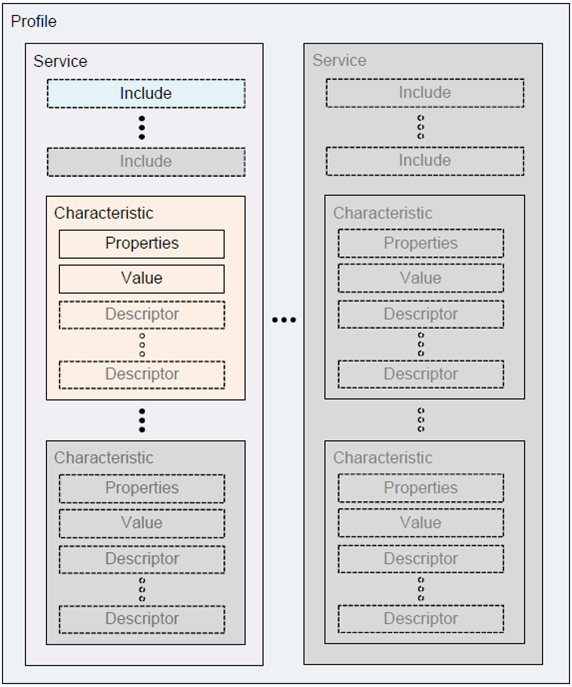
\includegraphics[width=0.6\textwidth,center]{fig/gatt}
\caption{Hierarki for GATT-profiler} %\todo{Kilde? \url{https://www.bluetooth.com/specifications/generic-attributes-overview}}
\label{fig:gatt}
\end{figure}

\subsubsection{Sikkerhet i BLE}
De største sikkerhetsproblemene til BLE generelt er passiv tyvlytting, \gls{mitm} og identitetssporing.
Bluetooth 4.0 ble annonsert i 2010, og er nå delvis utdatert når det gjelder sikkerhet. Alle paringsmetodene
til 4.0 og 4.1 kalles for \textit{LE Legacy Pairing}. 

For å unngå passiv tyvlytting, krypterer BLE dataen som sendes mellom to enheter med en sikker blokkchiffer (AES-CCM). Problemet oppstår
i nøkkelutvekslingen mellom de to enhetene. I den vanligste paringsmetoden i \textit{LE Legacy Pairing}, \textit{Just Works\texttrademark},
brukes en svak midlertidig nøkkel (nøkkelen er tallet 0). Dermed er det enkelt for en angriper å finne ut hva korttidsnøkkelen
blir med rå datakraft og gjetting. Andre paringsmetoder eksisterer, men disse trenger brukerinteraksjon eller andre trådløse protokoller (NFC).
De er imidlertid rimelig sikre mot \gls{mitm} \citep{eewiki_ble}.

4.2 introduserer \textit{LE Secure Connections}. I denne utgaven av Just Works\texttrademark-paring blir det kun generert
én langtidsnøkkel ved hjelp av Elliptic Curve Diffie Hellman asymmetrisk kryptering. Dette løser problemet med passiv
tyvlytting, men forbindelsen er fortsatt sårbar for \gls{mitm} siden autentisering mangler. Et lite tillegg til Just Works\texttrademark
der man sammenligner om to verdier er like gjør denne metoden sikker mot \gls{mitm} \citep{eewiki_ble}.

Etter at enhetene er paret, er det mulig å lagre nøklene på hver enhet slik at de kan gjenbrukes uten å gå igjennom hele
paringsprosessen på nytt. Dette kalles \textit{bonding}.

Bluetooth 5 som begynner å komme i produkter våren 2017, lover lengre rekkevidde og økt hastighet.

%https://electronics.stackexchange.com/questions/284056/can-ble-transactions-be-encrypted-without-pairing
%https://security.stackexchange.com/questions/100554/is-bluetooth-4-0-traffic-encrypted-by-default-design
%https://piratecomm.wordpress.com/2014/01/19/ble-pairing-vs-bonding/
%https://community.nxp.com/thread/332191

\subsection{Seriell kommunikasjon og GPIO}
Det er flere ulike kommunikasjonsprotokoller for å snakke med annen elektronikk og andre integrerte kretser.
Seriell kommunikasjon består, i sin enkleste form, av å sende og motta binærdata over en asynkron seriell datalink.
Figur \ref{fig:serial} viser oppsettet mellom to enheter. En seriell enhet må ha en port for å motta data (RX)
og en port for å sende data (TX).

\Gls{gpio} er et generisk tilkoblingspunkt på en datamaskin eller integrert krets. Det er et grensesnitt mellom enheten
og omverdenen som gjør det mulig koble til for eksempel knapper og lys. Tilkoblingspunktene kan være konfigurert som
input eller output. I output-modus kan tilstanden til et punkt være enten høy (typisk 5V eller 3.3V) eller lav (0V).
I input-modus leses også signalet som høyt eller lavt med en trekk opp- eller trekk ned-motstand, og kan dermed
brukes til \textit{interrupts}.
%\todo{Kilde: \url{https://www.raspberrypi.org/documentation/usage/gpio/}}

\begin{figure}
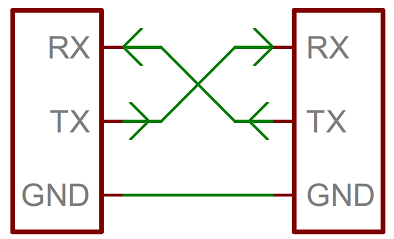
\includegraphics[width=0.5\textwidth,center]{fig/serial}
\caption{Seriell databuss}
\label{fig:serial}
\end{figure}

\section{Skyteknologi}

\subsection{Skybasert tingenes internett}
% \todo{Sikkerhet, personvern, kvalitetsattributter}

Det er flere skyløsninger på markedet med støtte for \gls{iot} og det er et marked i stor vekst.
Microsoft Azure IoT Hub og AWS IoT er allerede nevnt. IBM har en løsning kalt Watson Internet of Things Platform og
Google har Google Cloud IoT
som prøver å løse lignende problemer som Microsoft og Amazon.
Disse fire leverandørene dominerer markedet totalt. Data fra \citet{srg_cloud}
viser at AWS holder seg på 40 \% markedsandel i slutten av 2016, mens Microsoft,
Google og IBM har 23 \% markedsandel kombinert. De tre sistnevnte leverandørene vokser raskere enn AWS.

Dette prosjektet vil ta i fokusere på AWS IoT siden AWS er mest brukt i markedet i dag
og har et veldig modent økosystem. Azure IoT Hub nevnes kort. De fleste skysystemene tilbyr veldig like
løsninger.

\subsection{AWS IoT}
\label{sec:aws_iot}
Amazon sin \gls{iot}-løsning i skyen (\gls{aws} \gls{iot}) ble annonsert 9. oktober 2015.
Viktige aspekter av denne løsningen er \textit{AWS IoT Device SDKs} som tilkobler mot 
en \textit{device gateway}, og en \textit{rules engine} som tillater løsningen å integrere
mot andre AWS-tjenester. Se figur \ref{fig:awsiot_how} for arkitekturoversikt.
Denne arkitekturen likner veldig på den \citet{iot_harvard_smart} foreslo i kapittel \ref{ch:background}.

\textit{Thing registry} er en liste av alle enheter tilkoblet tjenesten, og en \textit{device shadow}
holder styr på tilstanden til en enhet som kan hentes eller modifiseres fra andre applikasjoner.

\begin{figure}
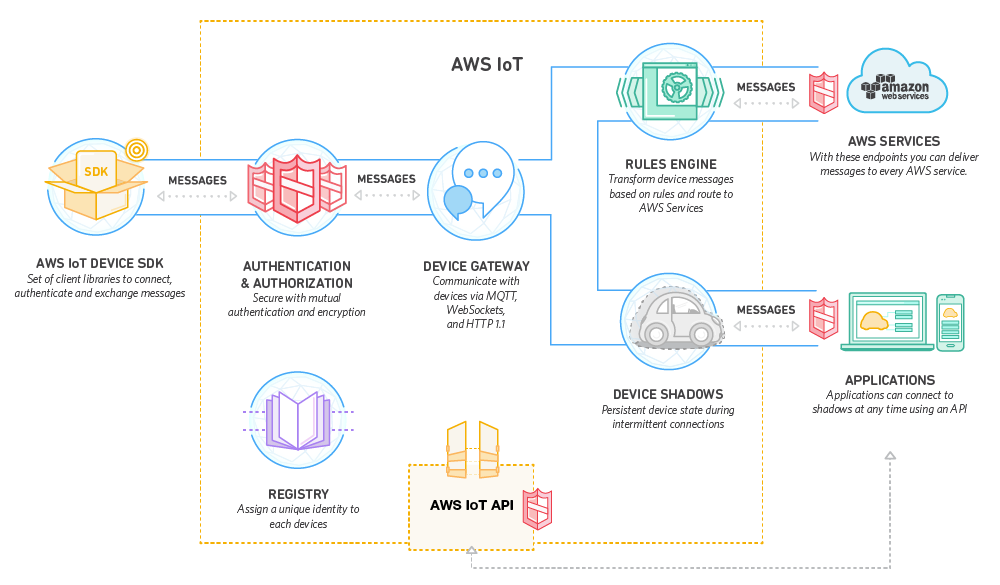
\includegraphics[width=1.0\textwidth,center]{fig/awsiot_how}
\caption{AWS IoT: Hvordan det virker \citep{aws_works}}
\label{fig:awsiot_how}
\end{figure}

\subsubsection{AWS IoT Device SDKs}
SDK-er er åpen kildekode på Github, og er tilgjengelige for embedded C, JavaScript (Node.js og nettleser),
Arduino Yún, Java, Python, iOS og Android \citep{aws_sdks}.

\subsubsection{Sikkerhet: Autentisering og tilgangskontroll}
AWS IoT tilbyr ende-til-ende-kryptering og gjensidig autentisering av alle meldinger med
\gls{tls} og klientside-X.509-sertifikater. Andre autentiseringsmetoder som Amazon sin egen SigV4-protokoll
er tilgjengelig også.

\subsubsection{Device gateway}
Device gateway fungerer som en skalerbar \textit{meldingsbroker} basert på publish-subscribe-mønsteret,
med støtte for MQTT (publish/subscribe), MQTT over WebSockets (publish/subscribe) og HTTP (publish).

\subsubsection{Rules engine}
Rules engine evaluerer innkommende meldinger etter at de passerer igjennom device gateway,
og videresender disse meldingene til resten av AWS-økosystemet avhengig av hvilke regler som er satt opp.
Dette betyr at meldinger for eksempel kan bli endret og sendt videre, lagret i en database, aggregert i en
dataanalyseløsning og brakt videre til andre skytjenester. \citet{aws_works} nevner AWS Lambda, Amazon Kinesis,
Amazon S3, Amazon Machine Learning, Amazon DynamoDB, Amazon CloudWatch og Amazon Elasticsearch Service som mulige
integrasjoner.

\subsubsection{Device shadows}
Alle enheter koblet til device gateway har en thing shadow som er et JSON-dokument
med nåværende tilstand og informasjon om enheten. En thing shadow til en ting er alltid tilgjengelig,
selv om enheten er koblet fra Internett. Den kan alltid bli hentet og endret over HTTP eller MQTT. En thing shadow
er identifisert med sitt unike navn. AWS IoT reserverer emnenavnene \textit{get}, \textit{update}
og \textit{delete} for å kommunisere med device shadows.

\subsubsection{Thing registry}
Et thing registry er en JSON-liste av alle tingene som er tilkoblet til tjenesten. Hver ting
har et navn, og kan valgfritt ha attributter i nøkkel-verdi-par, for eksempel modellnavn og watt
for en lyspære. Det er mulig å lage forskjellige typer ting og assosierere disse typene med en ting.

\subsection{Microsoft Azure IoT Hub}
Microsoft Azure IoT Hub (figur \ref{fig:azure_iot}) har mange av de samme egenskapene som AWS IoT med andre navn: \textit{cloud gateway},
\textit{device twins} og \textit{identity registry}. Autentisering gjøres enten med et unikt token per enhet eller med
X.509-sertifikater. I praksis tilbyr de to skyteknologileverandørene veldig mye av det samme.

\begin{figure}
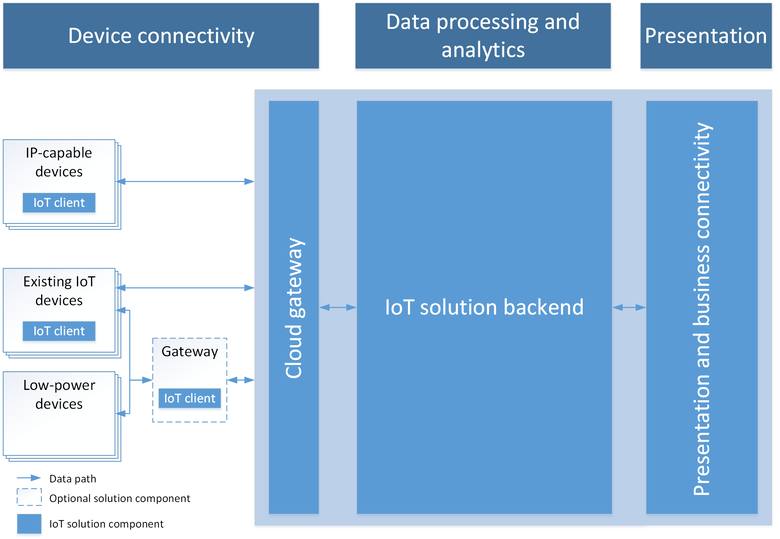
\includegraphics[width=1.0\textwidth,center]{fig/iot-reference-architecture}
\caption{Microsoft Azure IoT Hub: Løsningsarkitektur} % \todo{sitering?}
\label{fig:azure_iot}
\end{figure}

% \section{Utviklingsmiljø} \todo{Skal dette være med egentlig? Er det relevant å bable om Node.js her?}

\section{Prototypeplattform: Raspberry Pi Zero W}
Raspberry Pi Zero W er en liten og billig datamaskin med lavt strømforbruk lansert i februar 2017 (figur \ref{fig:pizero}).
Den har følgende spesifikasjoner: % \todo{https://www.raspberrypi.org/help/faqs https://www.raspberrypi.org/products/pi-zero-w/}
\begin{itemize}
    \item 1GHz, énkjerne-CPU
    \item 512MB RAM
    \item 802.11 b/g/n trådløs LAN
    \item Bluetooth 4.1 (BLE)
    \item Mini HDMI og USB On-The-Go-porter
    \item Micro SD-kortmodul
    \item HAT-kompatibel 40-pin header
    \item \textbf{Strømforbruk:} typisk 100mA i hvilemodus og maks 350mA under stress
    \item \textbf{Størrelse}: 65 mm × 30 mm × 5 mm
\end{itemize}

Figur \ref{fig:pizero_gpio} viser de ulike portene til \gls{gpio}-headeren. Det er flere kontakter for
jording, 5V, 3V, og noen porter kan brukes til seriell kommunikasjon og I2C i tillegg til \gls{gpio}.
Raspberry Pi Zero W kjører på Raspbian, et Debian-basert operativsystem laget spesielt for de ulike utgavene av
Raspberry Pi med Linux-kjernen i bunn..

\begin{figure}
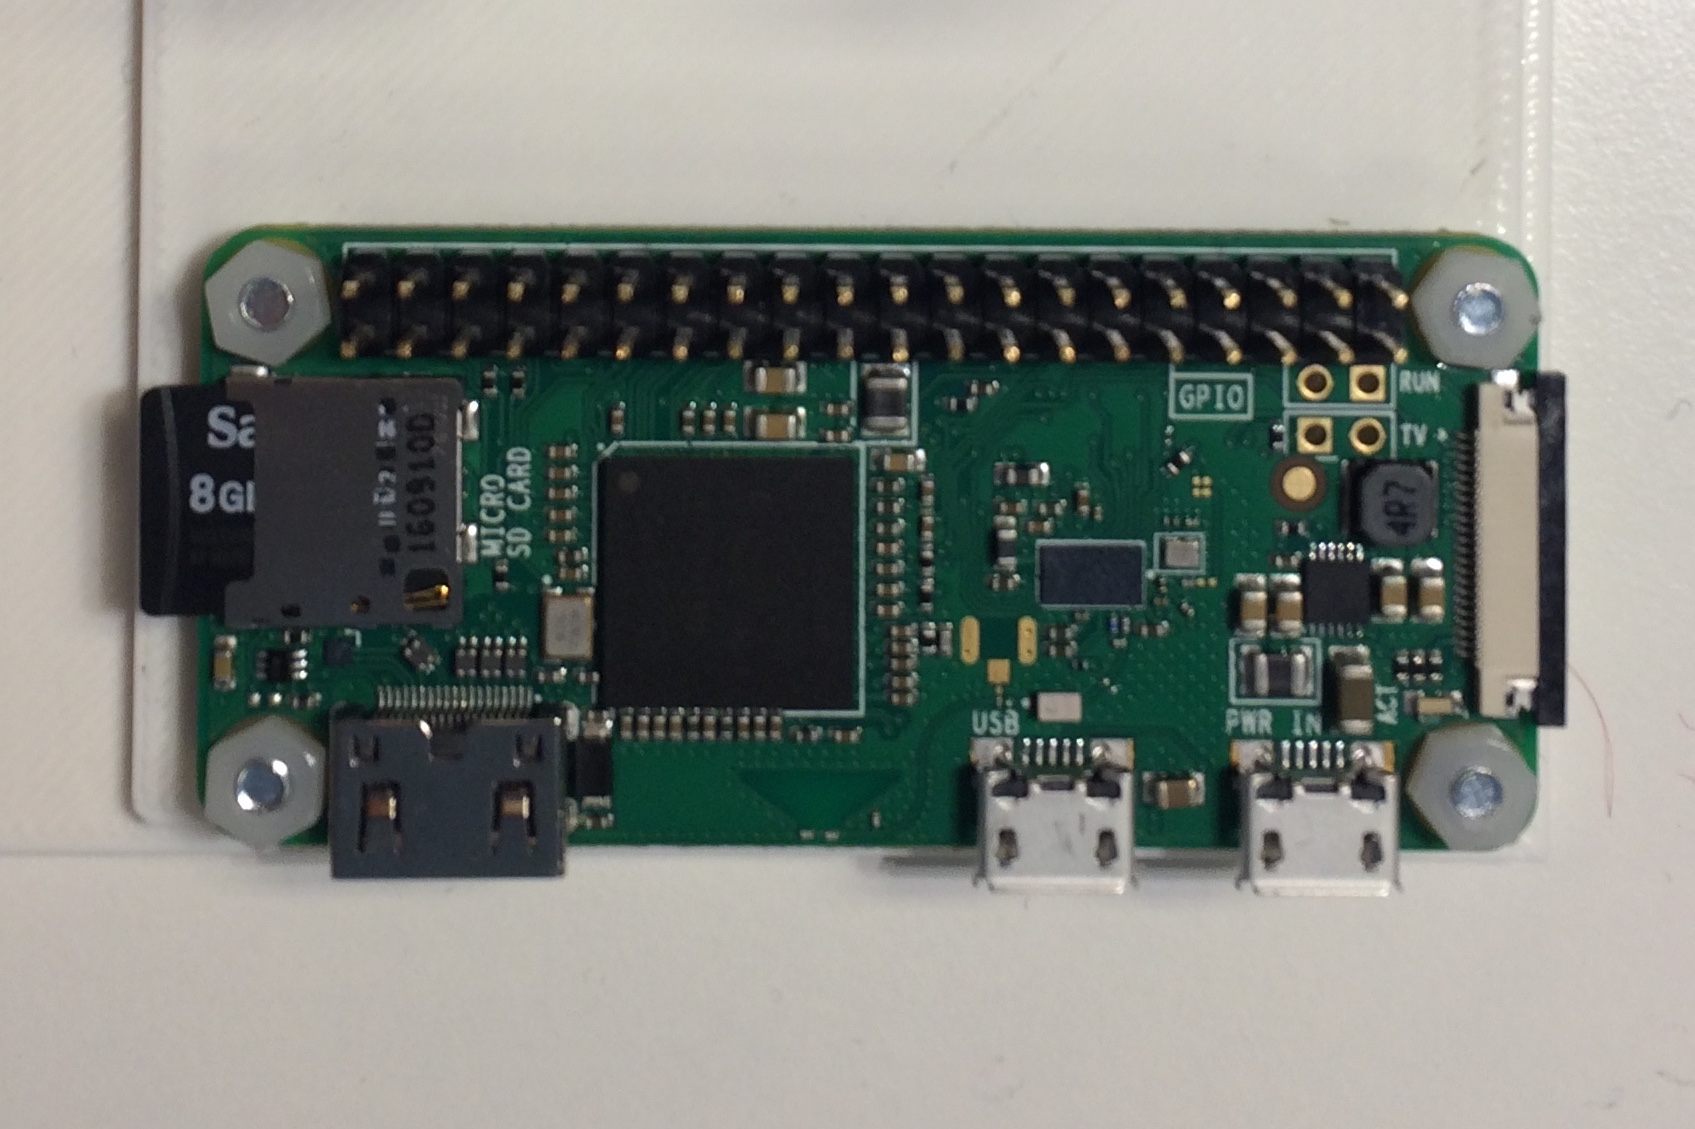
\includegraphics[width=0.8\textwidth,center]{fig/prototype/pi}
\caption{Raspberry Pi Zero W}
\label{fig:pizero}
\end{figure}

\begin{figure}
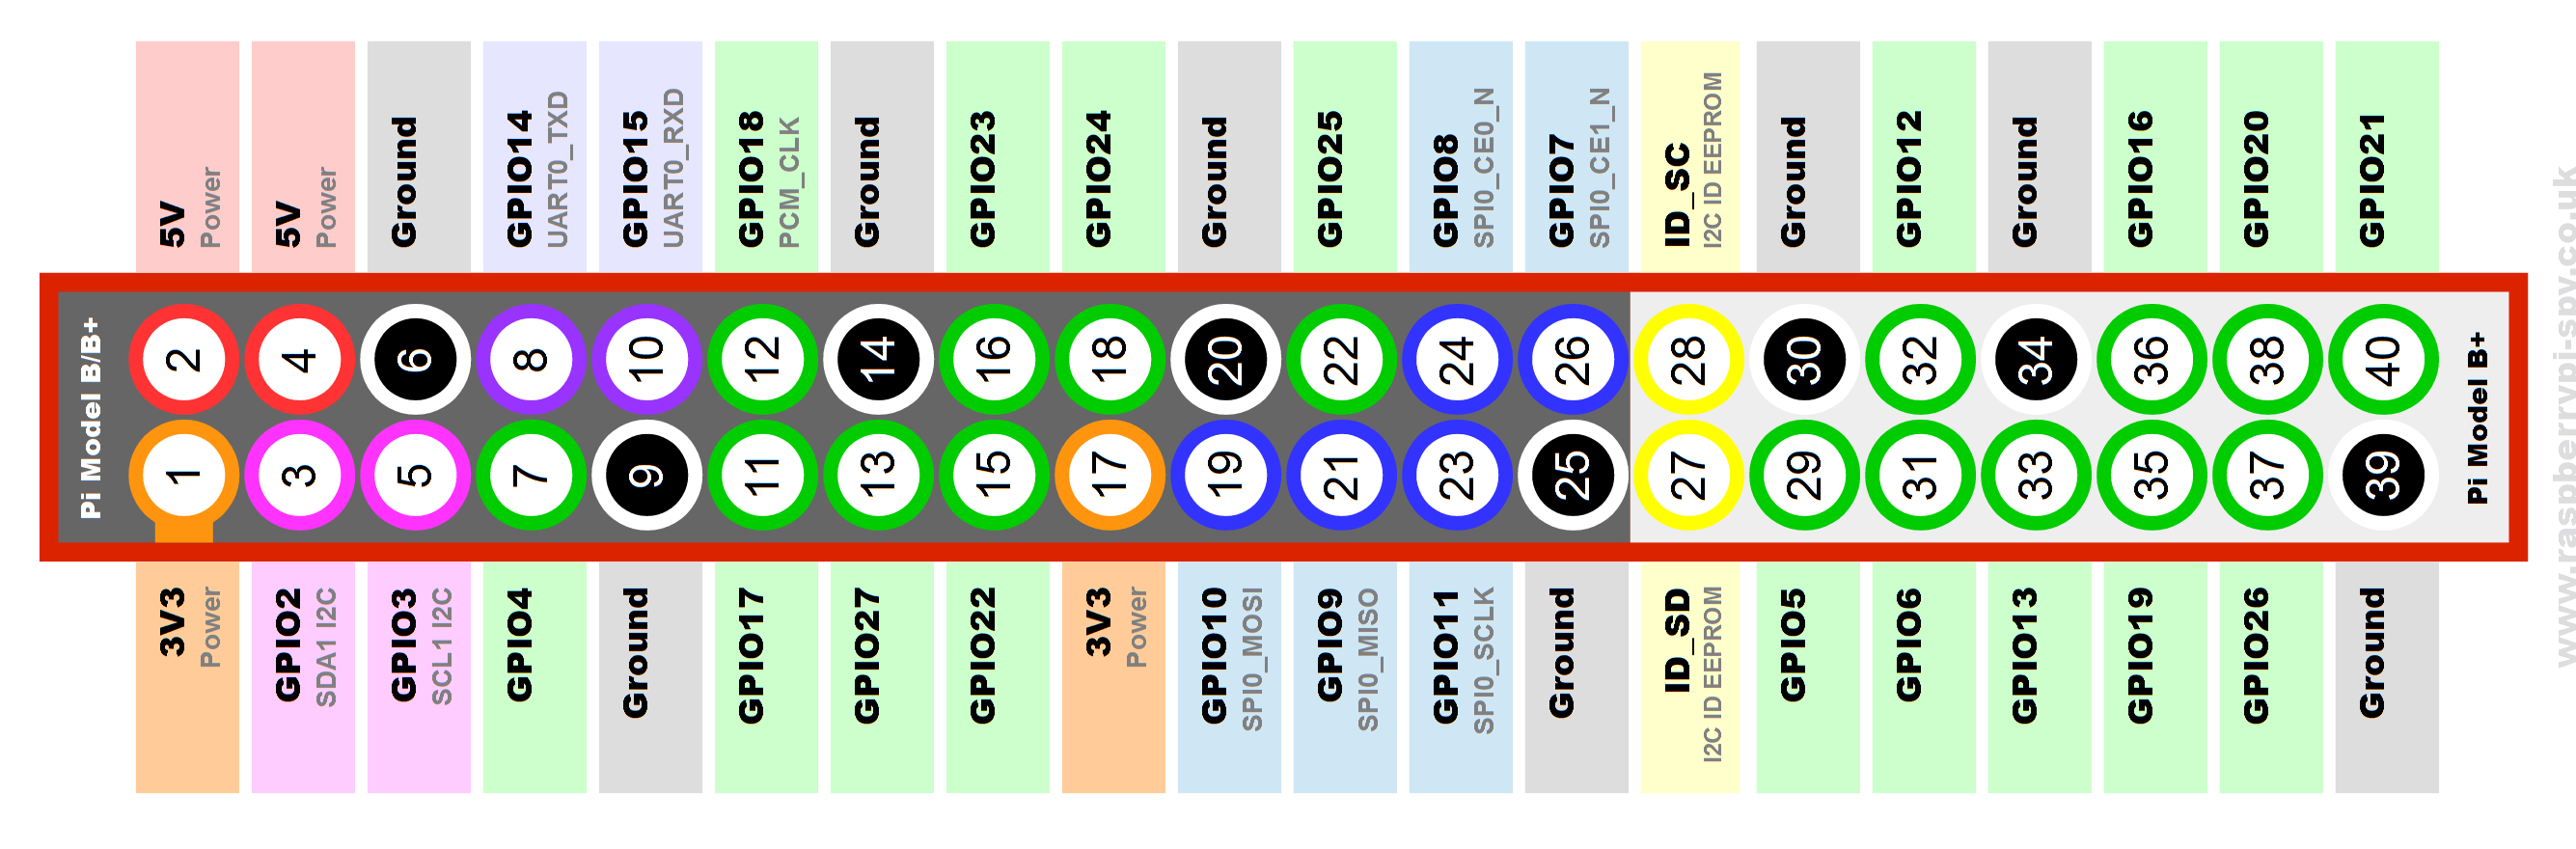
\includegraphics[width=1.0\textwidth,center]{fig/pizero_gpio}
\caption{Pi Zero W: GPIO header. Foto: \url{http://www.raspberrypi-spy.co.uk}}
\label{fig:pizero_gpio}
\end{figure}

\section{Sensorer og aktuatorer}
En sensor er en innretning som gir signal om en tilstand i den fysiske omverdenen. Eksempler
på sensorer kan være temperaturmåler, bevegelsessensor, ultralyd og trykknapp. Aktuatorer er innretninger som påvirker
den fysiske omverdenen på en eller annen måte, for eksempel lysdioder, buzzere og LCD-skjermer.
% https://www.ntnu.no/wiki/display/plab/1.+Generelt+om+aktuatorer+og+LED
% https://www.ntnu.no/wiki/display/plab/1.+Generelt+om+sensorer+og+trykknapper

\subsection{Pulsoksymeter}
Et pulsoksymeter er en sensor som måler oksygenmetning i blodet og pulsfrekvens.

Trondheim kommune lånte ut en Nonin 3230 (se figur \ref{fig:nonin-3230}) til bruk i denne masteroppgaven.
Nonin 3230 er et pulsoksymeter med støtte for \gls{ble} 4.0. Dette pulsoksymeteret ble anbefalt av \citet{austad2016sensorer}
i rapporten \textit{Sensorer til støtte for avstandsoppfølging}. De trakk fram at alle Nonins produkter
er klinisk validerte og at det er støtte for \gls{ble}. % @TODO OG BLABLA NOE MER

Nonin 3230 måler oksygenmetning fra 0 til 100\% og pulsfrekvens fra 18 til 321 slag per minutt. Den går på to
AAA-batterier, og er spesifisert for 2200 spotmålinger (25 sekunder per måling).

\begin{figure}
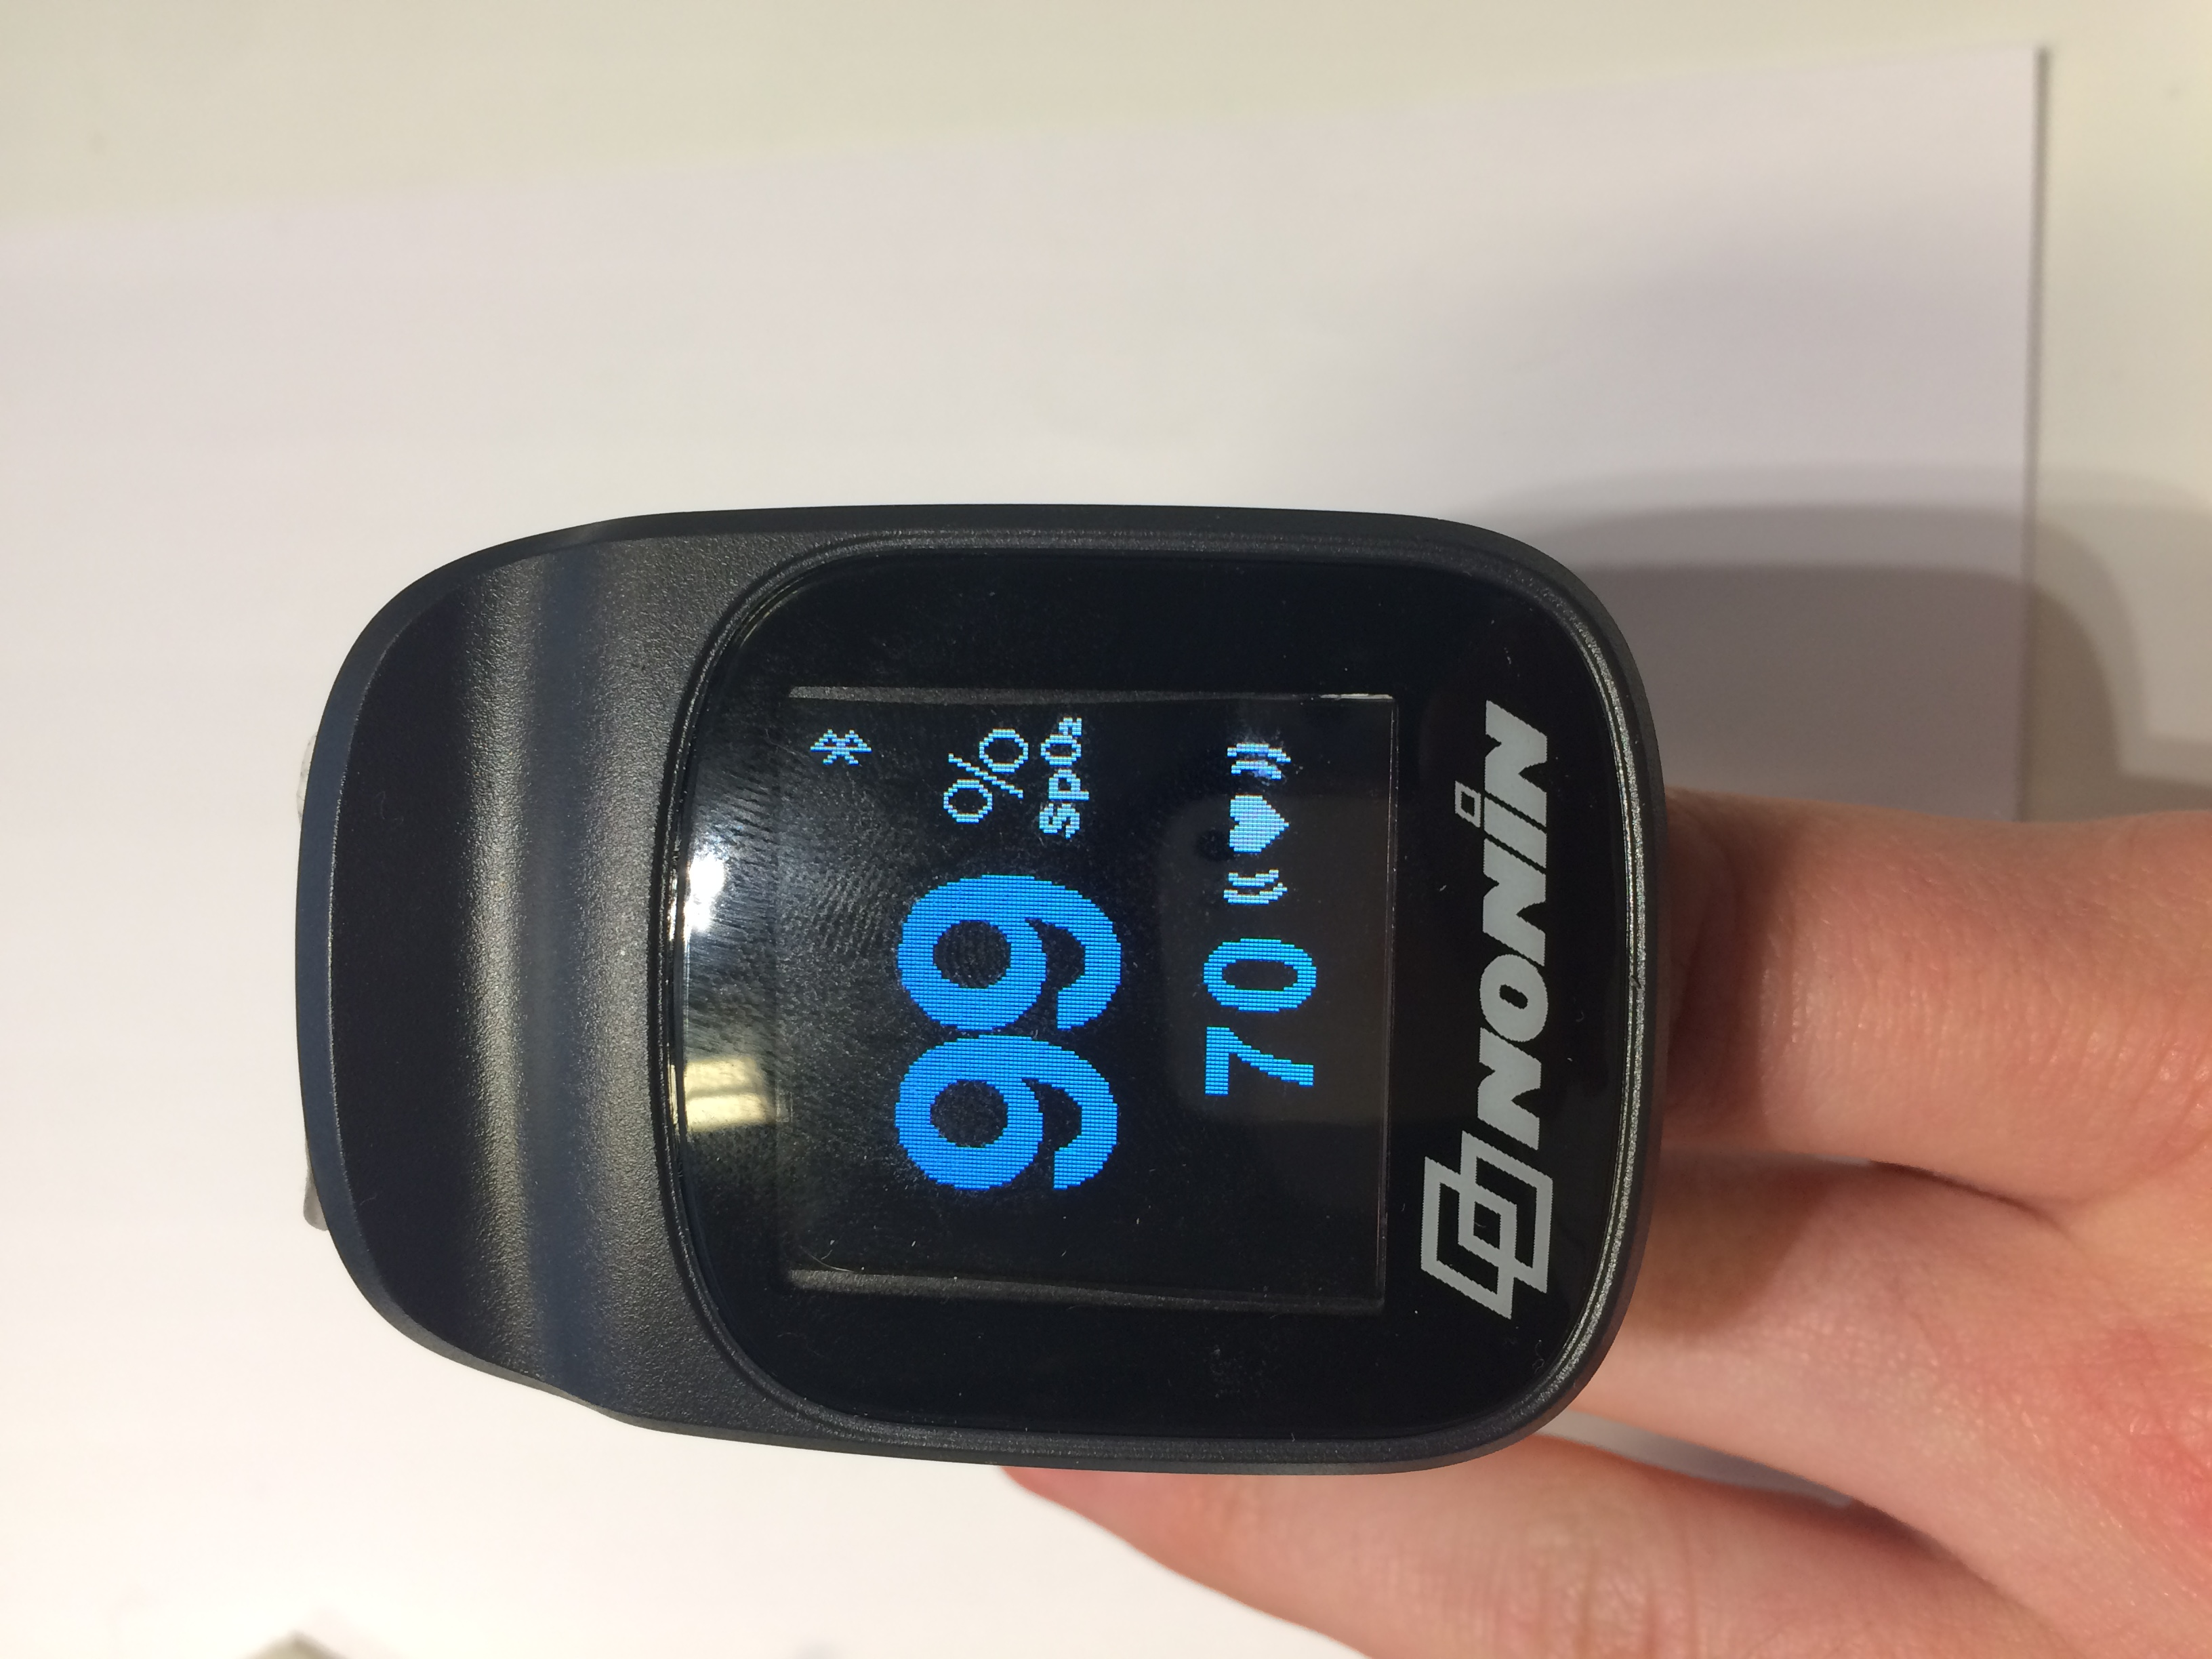
\includegraphics[width=0.75\textwidth, center]{fig/prototype/nonin3230ble}
\caption{Nonin 3230}
\label{fig:nonin-3230}
\end{figure}

%https://www.protocentral.com/sensors/1030-protocentral-pulse-oximeter-heart-rate-sensor-based-on-max30100.html
\subsection{Fingeravtrykksensor}
Fingeravtrykksensor er en sensor som kan prosessere et fingeravtrykk og verifisere og matche et avtrykk mot
et tidligere lagret bilde av avtrykket. I dette prosjektet er det blitt kjøpt inn sensor som heter GT-511C3 (figur \ref{fig:gt511c3}).
Prisen på denne sensoren er litt over 400 kr. Den tar i mot enkle kommandoer for å styre sensoren over seriell kommunikasjon.

\begin{figure}
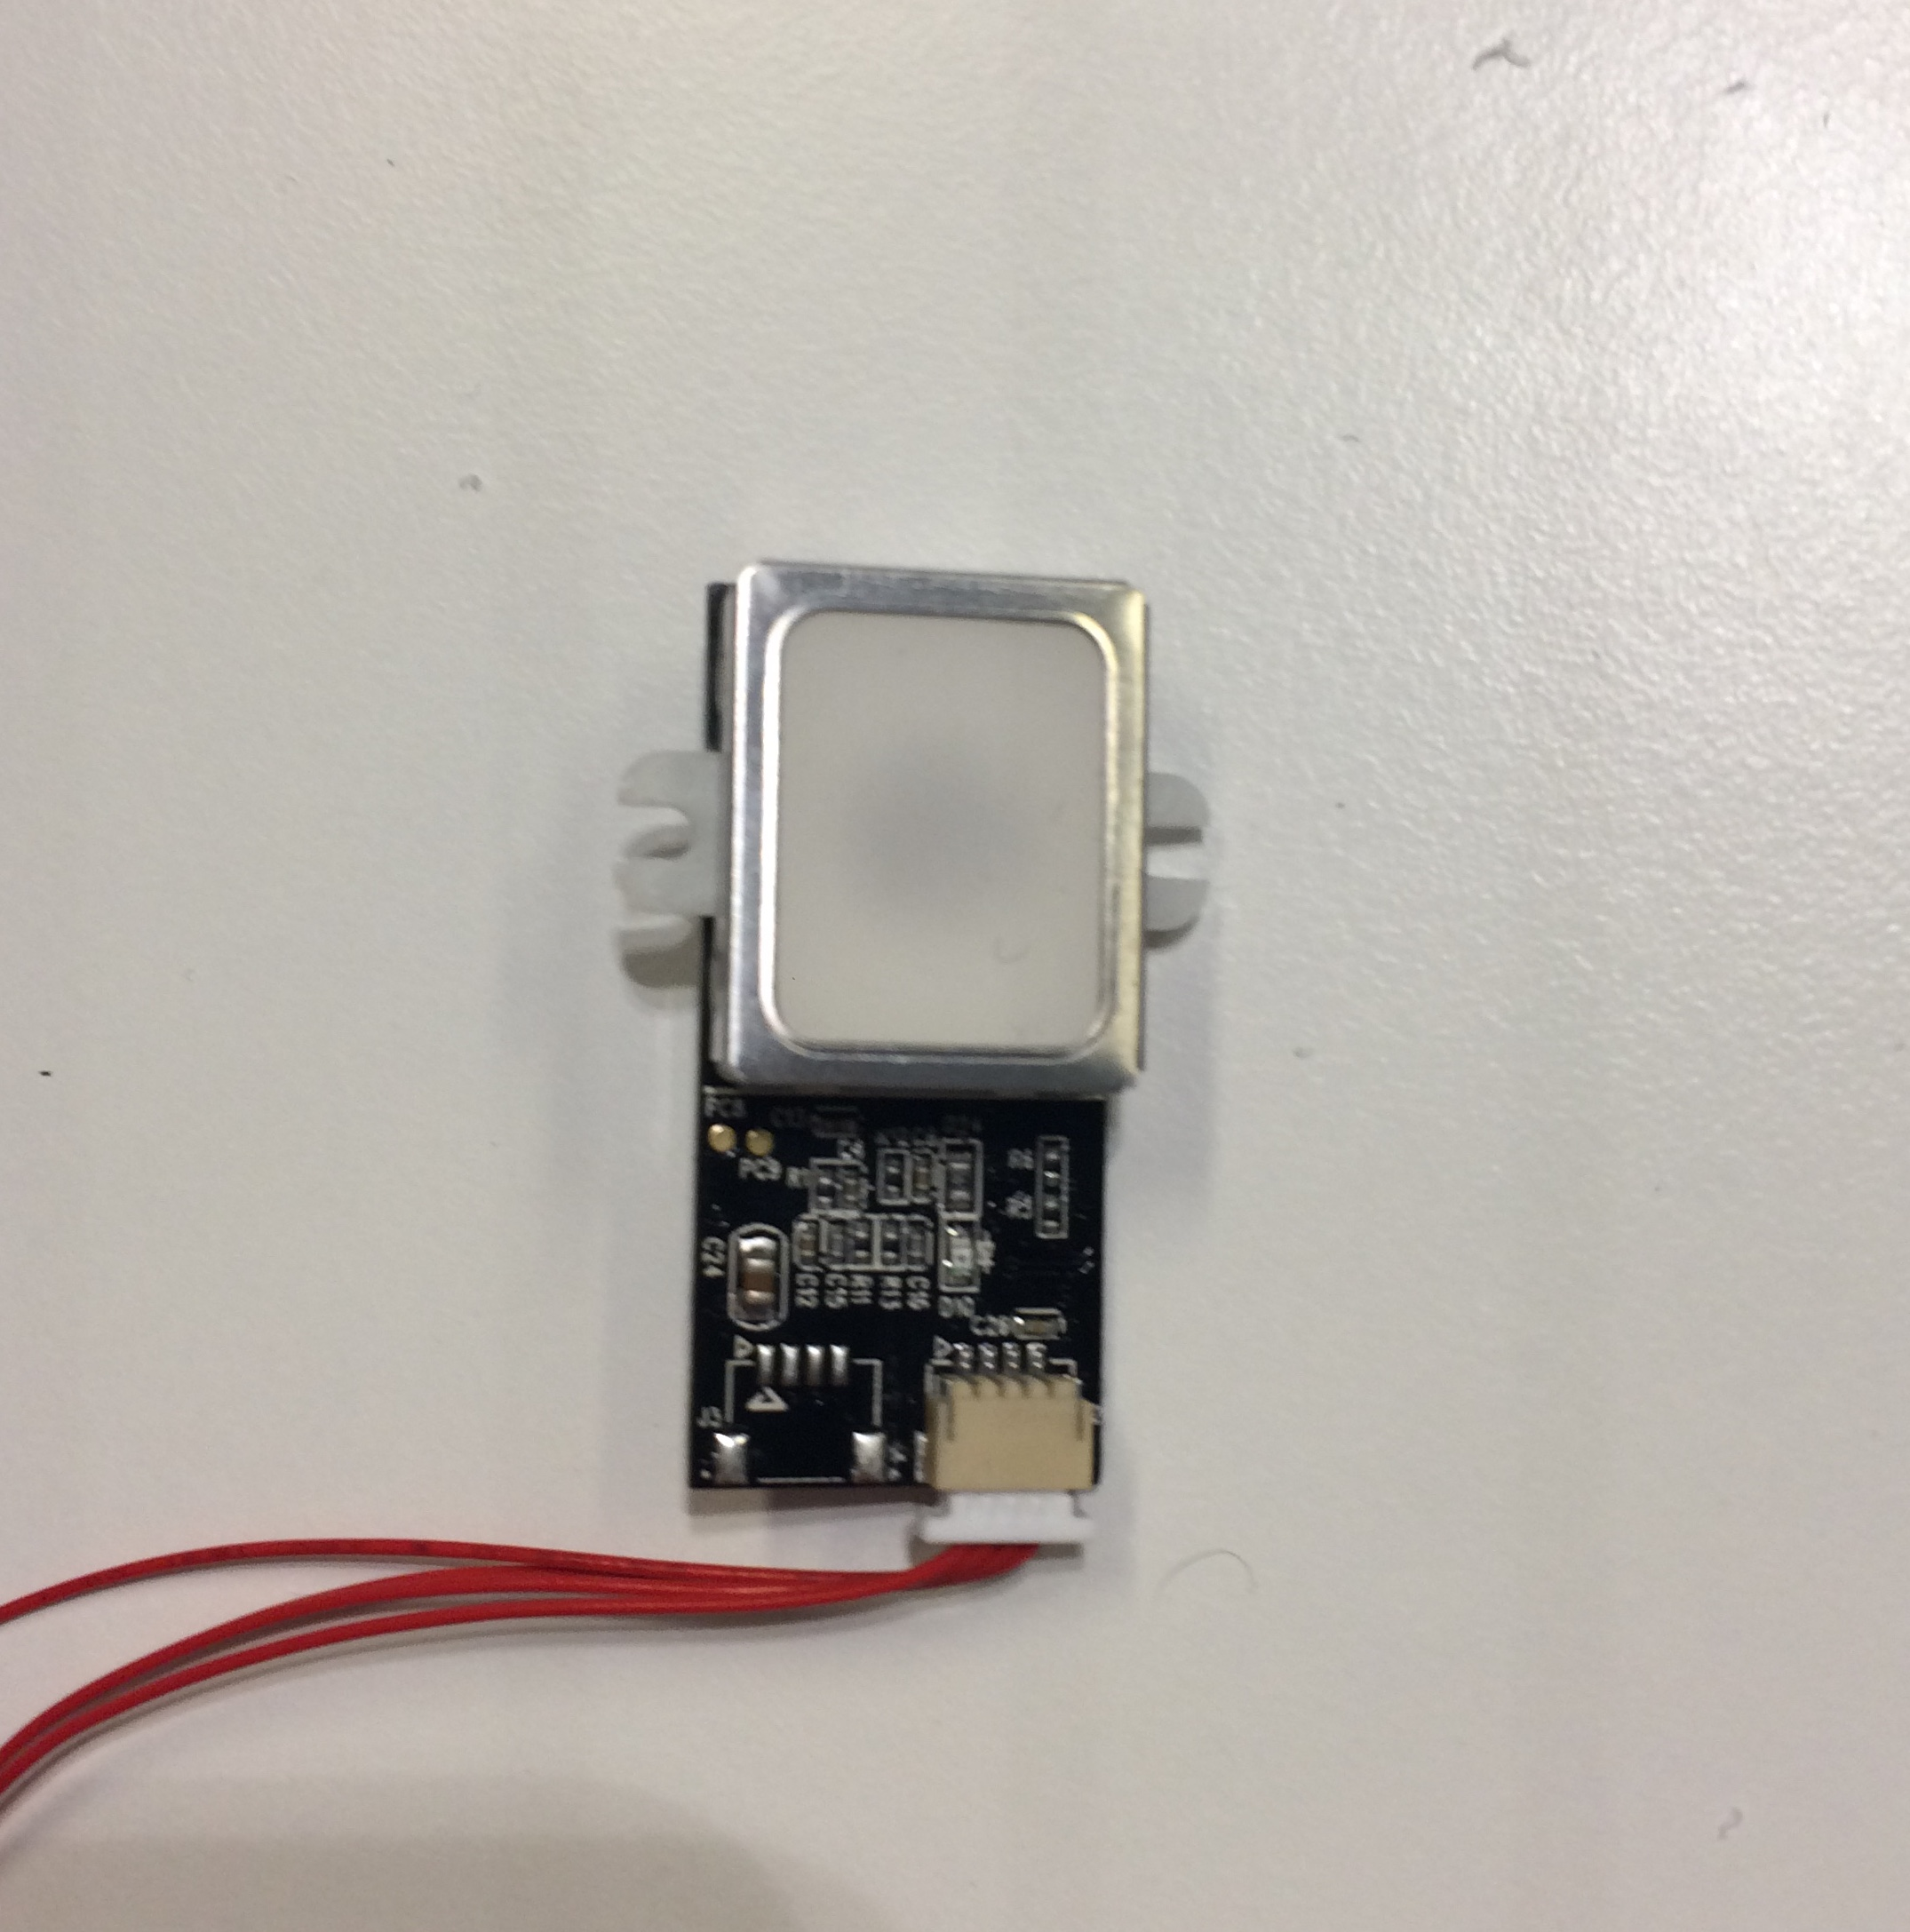
\includegraphics[width=0.55\textwidth, center]{fig/prototype/fingerprintsensor}
\caption{GT-511C3}
\label{fig:gt511c3}
\end{figure}

\subsection{Trykknapp og lysdioder}
Lysdioder er enkle aktuatorer som gir fra seg lys og kan styres programmatisk. I dette prosjektet brukes tre RGB-lysdioder og en hvit lysdiode.
RGB-lysdiodene trenger tre tilkoblingspunkter
for rødt, grønt og blått lys i tillegg til jording. RGB-lysdiodene må ha en motstand foran seg. Lysdiodene styres med pulsbreddemodulasjon i software.
Det brukes også en helt enkel trykknapp som er konfigurert til pullup, det vil si at verdien er 0 (LOW) når knappen trykkes ned
og 1 (HIGH) når knappen er åpen. Figur \ref{fig:lysdioder_motstander} viser noen av de ulike komponentene.

\begin{figure}
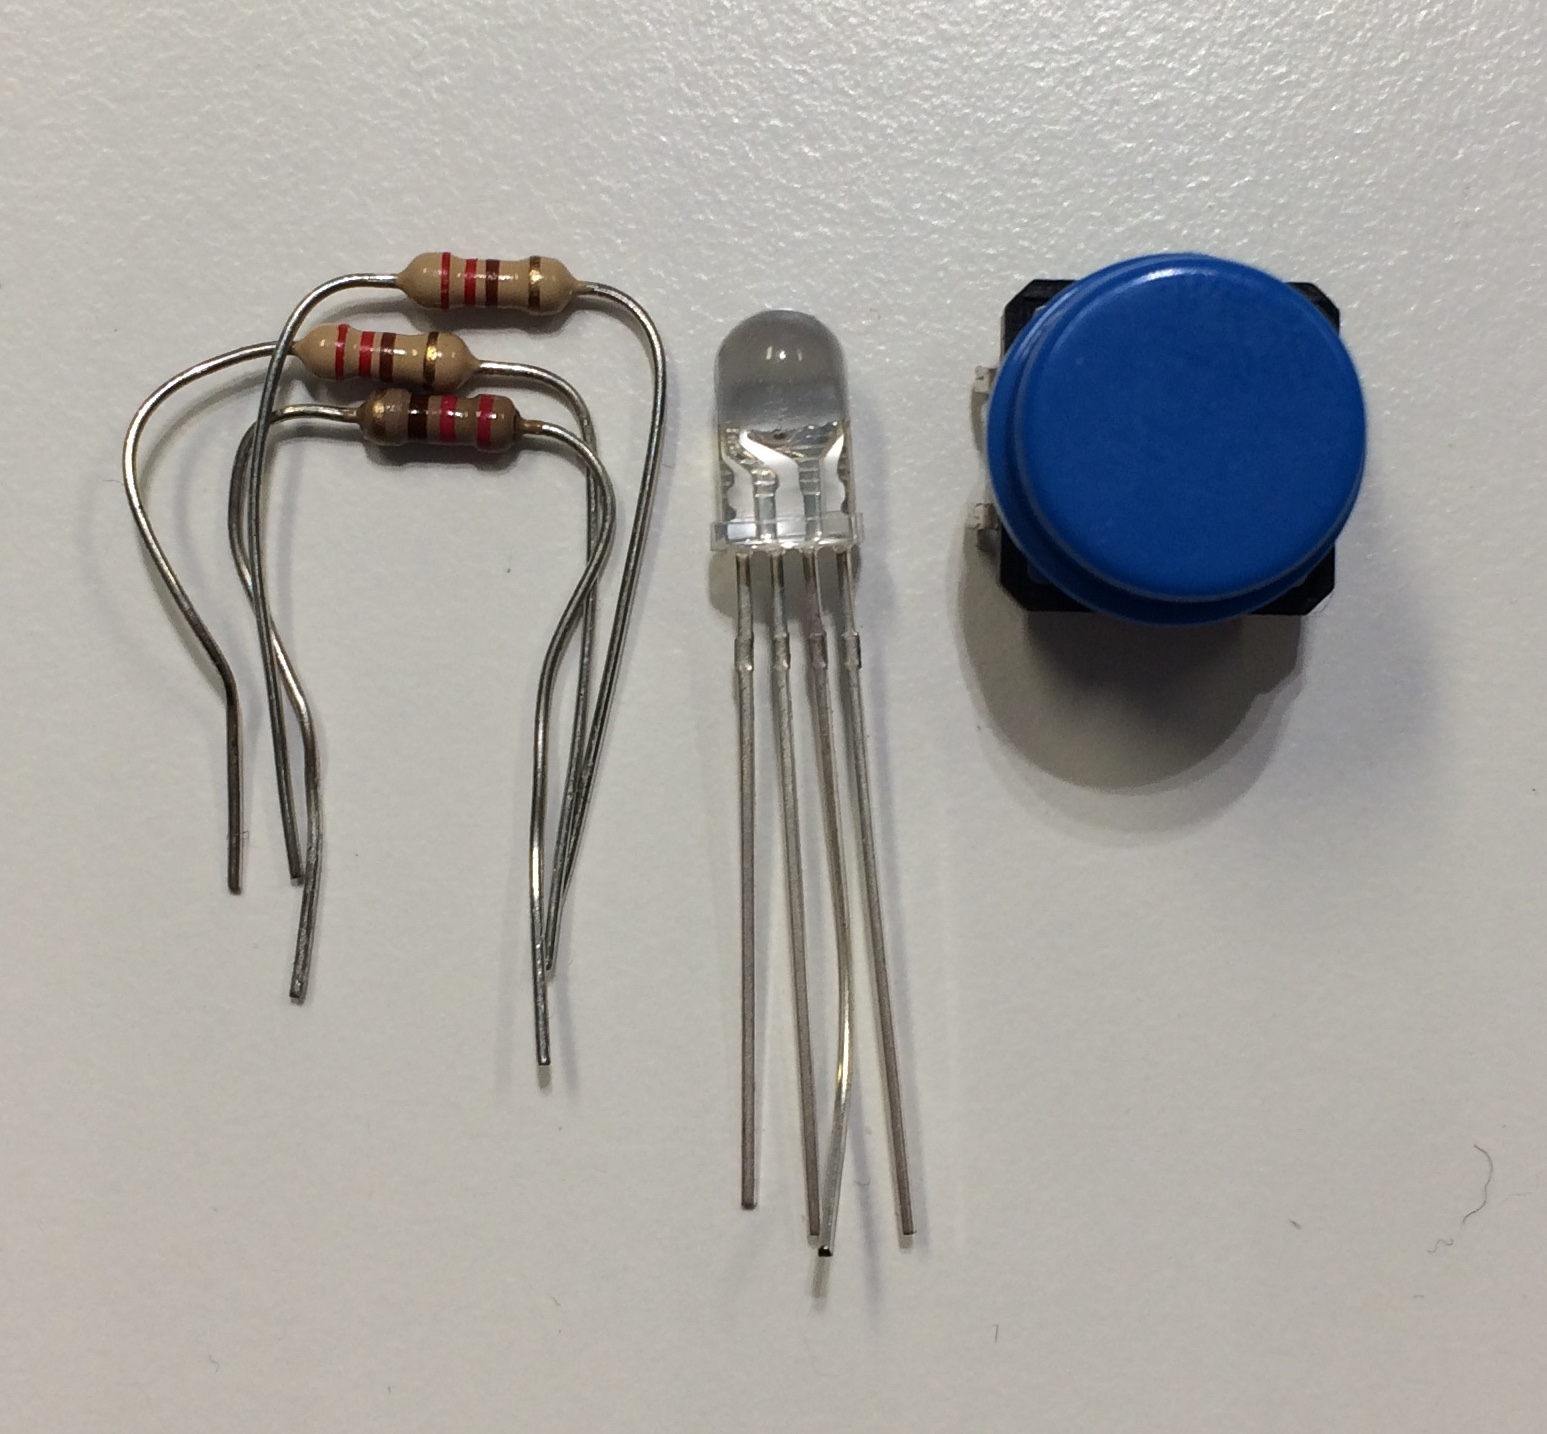
\includegraphics[width=0.55\textwidth, center]{fig/prototype/ledmotstandknapp}
\caption{RGB-lysdiode, motstander og trykknapp}
\label{fig:lysdioder_motstander}
\end{figure}
